\section{Introduction}

Traffic regulation or pollution measurement in water are example activities which require the constant presence of measuring agents over wide ---~and sometimes hard to access~--- areas.
In such cases, as it is not feasible to send people on site to run measurements, \wsns are used.
They are made of small devices, sometimes dropped on the spot by helicopter, tasked with gathering data on their physical environment.
Sensors are able to exchange data through wireless communications.
Useful data is typically centralized by a \bs, which acts as an interface between the network and the user.

As they are often used in hostile environments with no human assistance, sensors are generally able to self-organize and to form a consistent network.
But they also embed cheap hardware, as it may be hard, if possible at all, to fetch them once their life cycle is over.
Consequently, they have restricted resources: low computational capabilities and low available memory.
They also have limited energy%ONDEMAND \cite{BF12}
in a single-use battery.

\Wsns are used for many applications%ONDEMAND \cite{RFH12,FH13}
, some of them being crucial.
For instance there is a lot at stakes when sensor networks are used for watching forests for fires, for measuring the nuclear activity degree in sensitive areas, or for military operations over battlefields.
In this context, bringing security guaranties ---~including availability~--- to the network becomes essential.

Based on former studies (see Section~\ref{ea:sec:related}), the present one relies on the use of monitoring nodes (or ``\cns'') to protect a \wsn again various \dos attacks.
Actually, it focuses on the election process of those control nodes.
Our approach consists in taking energy into account at this step, in order to obtain an even better load balancing.
We propose to designate the sensors for the \cn position according to their residual energy, but we show that several problems occur with deterministic election.
Indeed compromised nodes could see a flaw to exploit in order to take over the \cn role and decrease the odds of being detected by announcing high residual energy.
We address this issue by introducing a second role of surveillance: we choose ``\vns'' responsible for watching over the \cns and for matching their announced consumption against mathematical model.
We also recommend that every node in the cluster be monitored by at least one \cn to prevent all the \cns to be elected inside the same spatial area of the cluster at each election iteration.

\section{Related work}
\label{ea:sec:related}

For sensitive operations involving the deployment of a \wsn, all security aspects of the network must be reviewed.
WSN-addressed protocols to provide data privacy\cite{OX09} and authentication\cite{SOBMCN11} have been subject to deep research investigation, and led for example to the proposal of mechanisms for secure data aggregation without persistent cryptographic operations\cite{WDSX07} or for authenticated broadcast such as $\mu$TESLA\cite{PSWCT02}.
But cryptography is of no use if the network is down: in this paper we focused on resistance against \dos (DoS) attacks.

Indeed there are many existing attacks able to compromise the good working of a \wsn.%ONDEMAND \cite{ZJ09}.
Several mechanisms have been proposed to detect it and to provide countermeasures\cite{SSS11}. %ONDEMAND ,SSF13}.
Many consist in the implementation of trust based mechanisms\cite{MC10,F-GRL07} with agents applying set of rules\cite{RKKK13} on traffic to attribute a trust value to each of the nodes in the network.
In particular, Lai and Chen\cite{LC08} proposed to elect control nodes to monitor the traffic in clustered networks and to detect and react to \dos attacks.
Clustered networks are partitioned into clusters \via algorithms such as \leach\cite{HHT02}.
One \ch (\CH) per cluster is responsible for gathering data from its peers, for aggregating and sending it to the \bs.
The \CHs are the only nodes to use long range (and expensive) transmissions to reach the \bs.
Clustering enables to preserve energy for the sensing nodes and offers an easier management of the nodes.
In our case, all nodes of a cluster can reach their \ch directly (\emph{1-hop transmission}), as on \figurename~\ref{ea:fig:wsn}.
\begin{figure}[h]
    \centering
    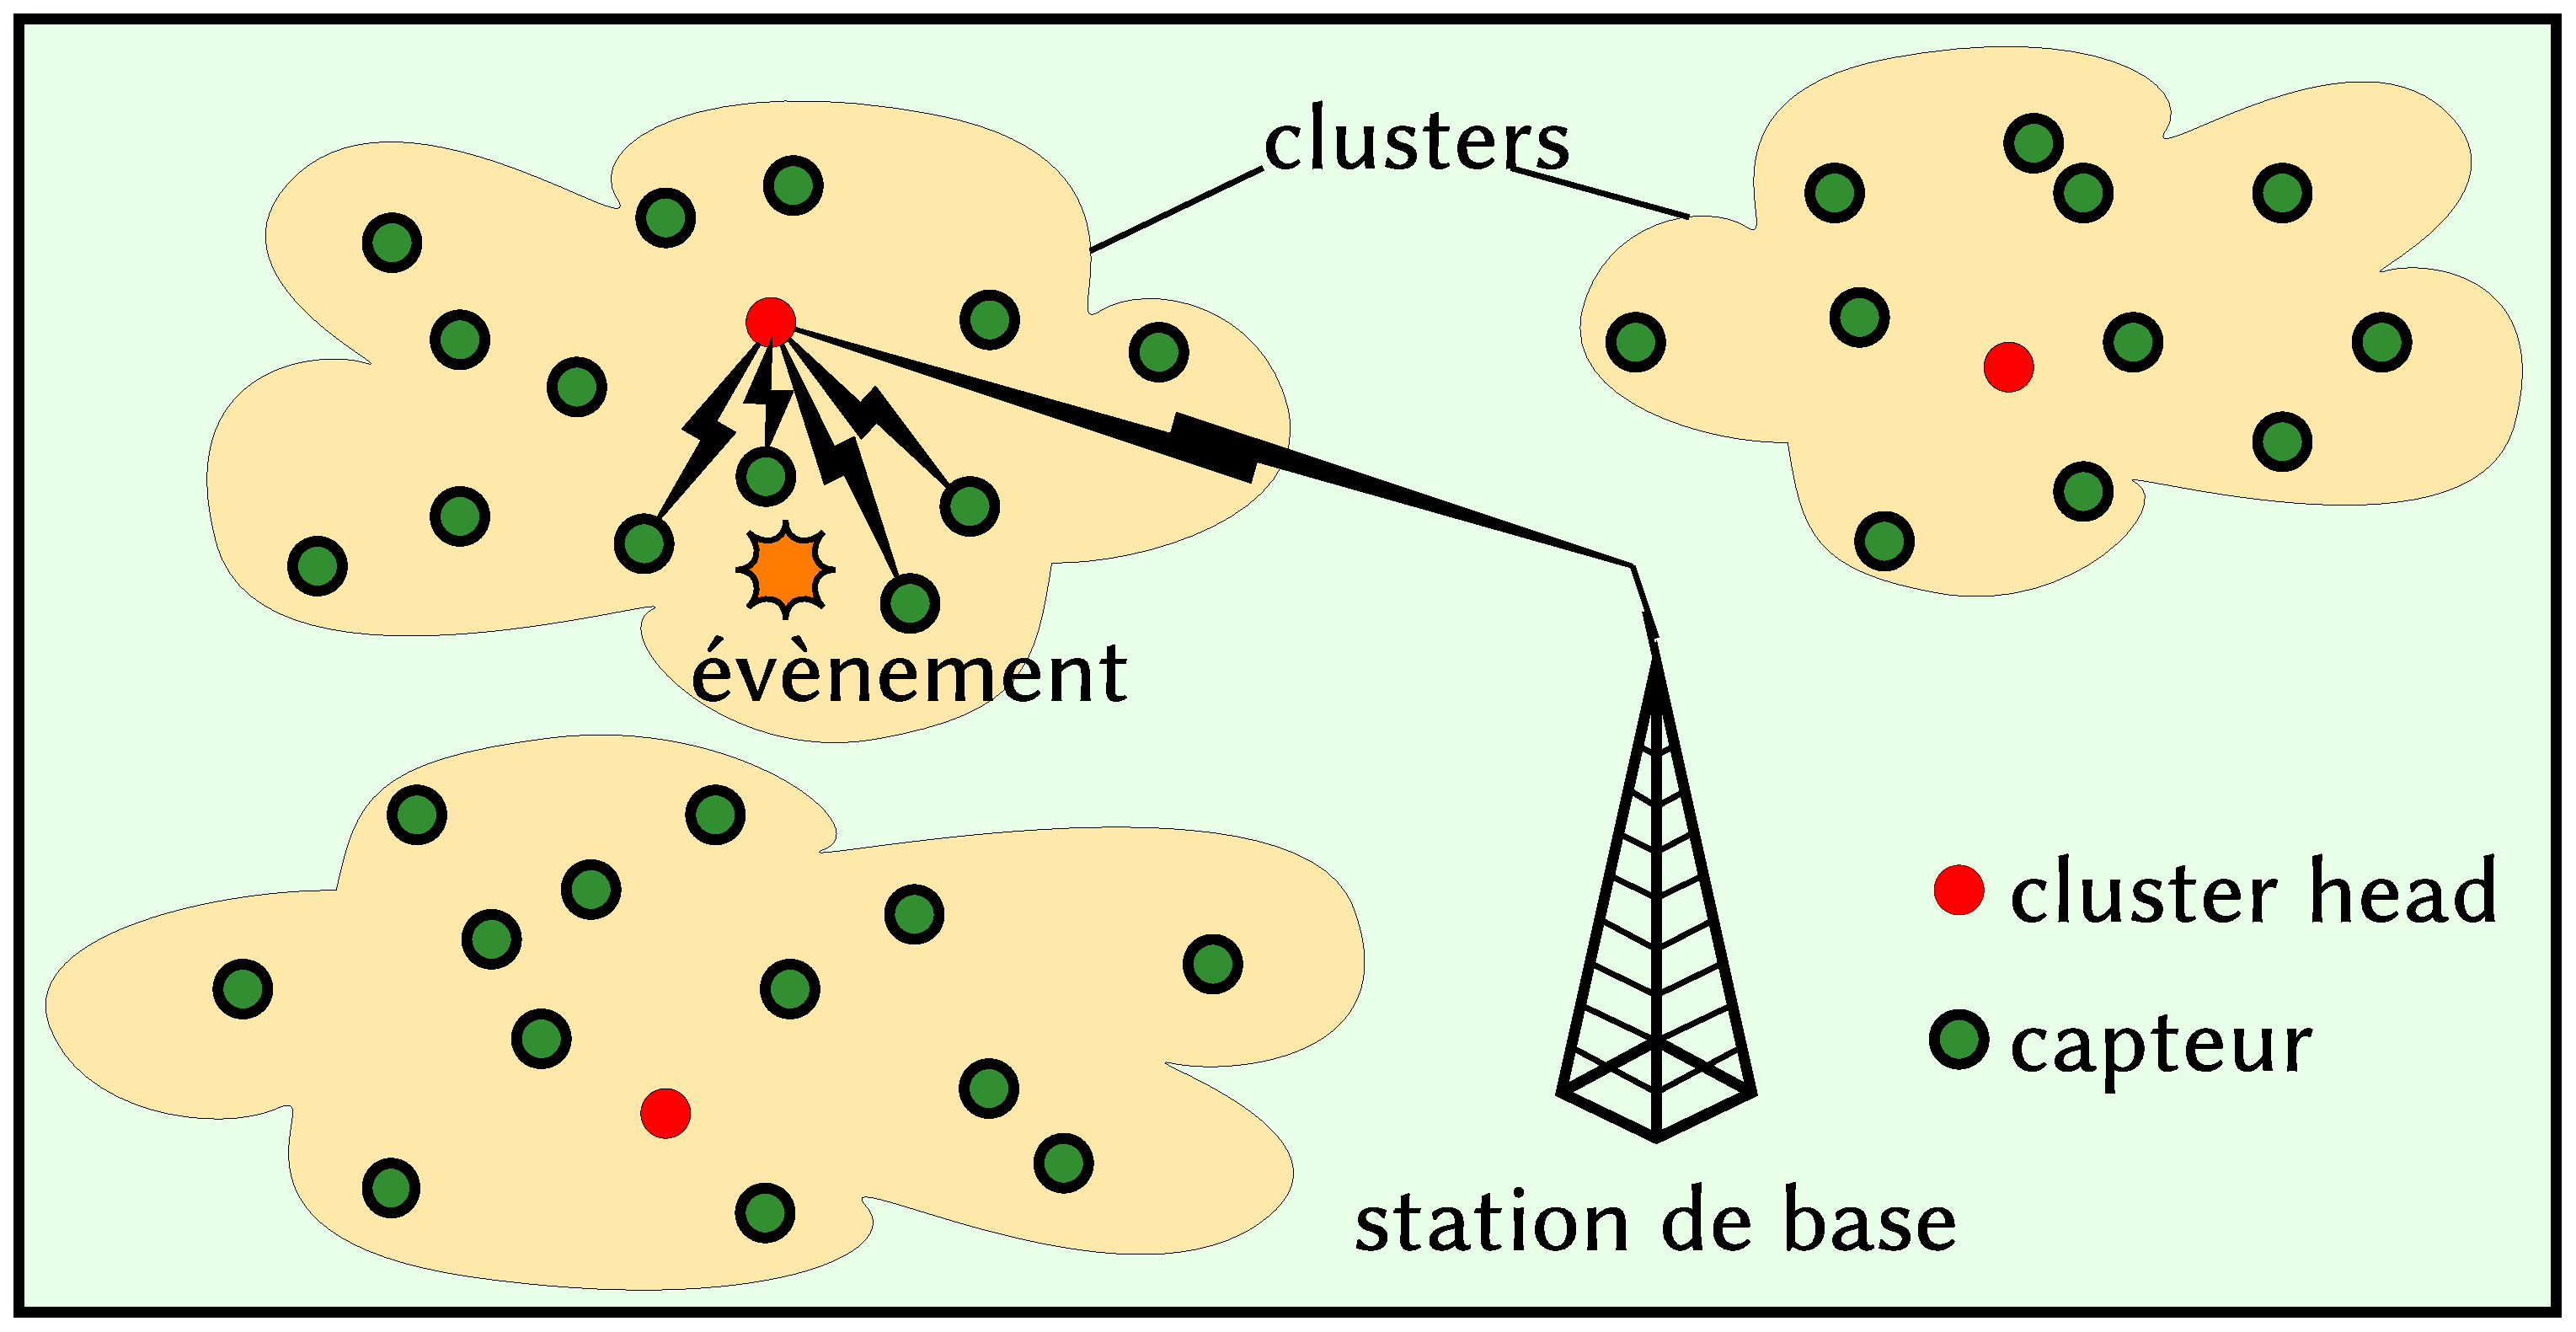
\includegraphics[width=0.8\linewidth]{\chapterfig/WSN.eps}
    \caption{Clustered wireless sensor networks scheme}\label{ea:fig:wsn}
\end{figure}

Control nodes are elected among the non-\ch nodes of a cluster.
We will call them \cns from now on.
They are responsible for listening to the traffic and detecting nodes whose emitted traffic exceeds a given threshold value.
These abnormal behaviors are reported to the \ch.
On reception of reports from several distinct \cns (to prevent false denunciation from a compromised node), the \CH virtually excludes the suspicious node from the cluster.
Although the method is efficient for detecting rogue nodes, the authors do not give details of the election mechanism to choose the \cns.
Also, there is no mention in their study of renewing the election in time, which causes the appointed \cns to endorse a heavier energy consumption on a long period.

In a first attempt to bring load balancing to this solution, we propose in other papers\cite{GMT12,BMM13} to reiterate the election periodically.
Simulations show a better load repartition among the cluster, but at this time our focus was not on designing an energy efficient election process for the \cns.
This is the purpose of the current study.
